\documentclass[10pt,conference,compsocconf]{IEEEtran}

\usepackage{cite}
\usepackage{amsmath,amssymb,amsfonts}
\usepackage{graphicx}
\usepackage{booktabs}
\usepackage{url}
\usepackage{hyperref}
\usepackage{fontawesome5}

\begin{document}

\title{Early Detection of Myocardial Infarction Risk: End-to-End Regularized Linear Classification on the BRFSS Survey}

\author{
  \IEEEauthorblockN{Jakob Fürst, Seyyed Erfan Mousavian, Maryam Tavasolinaeini}
  \IEEEauthorblockA{Students at EPFL, Lausanne, Switzerland\\
  Email: \{jakob.furst, erfan.mousavian, maryam.tavasolinaeini\}@epfl.ch\\
  \vspace{4pt}
  \href{https://www.aicrowd.com/challenges/epfl-machine-learning-project-1/submissions/338235}{AIcrowd Submission ID: 338235} \qquad 
  \href{https://github.com/jokobus/EPFL_CS433_project1}{GitHub: jokobus/EPFL\_CS433\_project1}
  }
}

\maketitle

\begin{abstract}
Cardiovascular disease (CVD), notably myocardial infarction and coronary heart disease (MICHD), is the leading cause of mortality globally. Early risk assessment via non-invasive lifestyle surveys enables timely clinical prevention. In this work, we build an end-to-end machine learning system to predict personal MICHD risk ($\_MICHD \in \{-1, +1\}$) from 328,135 patient records across 321 features in the CDC Behavioral Risk Factor Surveillance System (BRFSS 2015). Implemented strictly from first-principles NumPy without external ML toolboxes, our approach tackles two central hurdles: extensive survey missingness and severe class imbalance (8.83\% positive prevalence). We introduce an optimized pipeline combining domain code recoding, high-yield screening feature retention, ternary encoding, discrete one-hot expansion, clinical interaction terms, and a 5-fold stratified cost-sensitive Ridge Regression ensemble solved via zero-copy matrix subtraction. On full 5-fold cross-validation, our pipeline achieves an $F_1$ score of 0.4302 (87.48\% accuracy), which yields an official test performance of $F_1 = 0.444$ and 87.8\% accuracy on the unseen AIcrowd competition test set (Submission \#338235), substantially outperforming standard thresholding ($F_1 = 0.0096$) and linear baselines ($F_1 = 0.4069$).
\end{abstract}

\section{Introduction}
Cardiovascular diseases cause an estimated 17.9 million deaths annually~\cite{who2021cvd}. Identifying high-risk individuals through accessible health surveys offers substantial preventative utility before acute cardiac events occur. The Centers for Disease Control and Prevention (CDC) conducts the Behavioral Risk Factor Surveillance System (BRFSS), an annual telephone survey recording chronic health conditions, health practices, and behavioral risk factors across U.S. residents~\cite{cdc2015brfss}.

We frame this challenge as binary classification: predict personal diagnosis of myocardial infarction or coronary heart disease ($\_MICHD \in \{-1, +1\}$) from 321 survey features. This task poses two severe practical difficulties:
\begin{enumerate}
    \item \textbf{Survey Missingness \& High Dimensionality:} Out of 321 raw features, 147 contain over 50\% missing entries due to state-optional modules. Naive omission or crude filling introduces severe noise or collinearity.
    \item \textbf{Extreme Class Imbalance:} Only 28,975 respondents (8.83\%) reported positive MICHD history, versus 299,160 negative cases (91.17\%). Under this skew, standard classifiers optimizing raw accuracy default to the majority class, attaining a deceptively high 91.2\% accuracy but a near-zero $F_1$ score and zero clinical diagnostic value~\cite{he2009learning}.
\end{enumerate}
Here, we develop a transparent, fully reproducible NumPy pipeline, benchmark the core lecture algorithms, and systematically evaluate the impact of each preprocessing and modeling choice.

\section{Data Preprocessing \& Feature Engineering}
\label{sec:preprocessing}

Raw telephone survey responses require principled preprocessing to preserve signal while maintaining numerical stability:

\textbf{1) Domain Special Code Cleaning:} BRFSS encodes non-linear responses using special integer tokens. Count features (\texttt{PHYSHLTH}, \texttt{MENTHLTH}, \texttt{POORHLTH}) use code 88 to denote 0 days (none); alcohol frequency (\texttt{ALCDAY5}) uses 888 for 0 drinks. Treating these values as continuous severely distorts linear relationships. We recoded 88 and 888 to 0.0, and mapped refusal/uncertainty codes (7, 9, 77, 99, 777, 999, 9999) to NaN.

\textbf{2) Strategic Retention of Screening Features:} Discarding all features with $>50\%$ missing values discards the most predictive clinical risk factors. Questions such as daily aspirin therapy (\texttt{CVDASPRN}, $|r|=0.273$), blood pressure medication (\texttt{BPMEDS}, $|r|=0.213$), and physician advice (\texttt{DRADVISE}) were only administered in optional modules or conditional on high risk. We retained core survey features alongside these high-yield screening modules (up to 98\% missingness), capturing 188 raw predictors.

\textbf{3) Ternary Encoding for Binary Items:} For binary yes/no questions, responses are coded $\{1, 2\}$. We mapped $1 \to +1.0$ (Yes), $2 \to -1.0$ (No), and unasked/NaN $\to 0.0$ (neutral). This allows linear weights to add or subtract risk directly relative to the population baseline.

\textbf{4) Categorical One-Hot Expansion:} Ordinal/discrete survey questions exhibit non-linear step responses. We one-hot encoded discrete features with cardinality 3--10 and age categories (\texttt{\_AGEG5YR}, 14 levels), dropping one level per feature to prevent exact multicollinearity. This enables linear models to learn arbitrary monotonic or non-linear risk curves across age groups, general health ratings, employment status, and smoking categories.

\textbf{5) Clinical Interactions \& Mobility Disentanglement:} Multiplicative cardiovascular interactions compound risk. We constructed interaction pairs combining age, hypertension, diabetes, smoking, and sex. Importantly, mobility impairment (\texttt{DIFFWALK}) was crossed with diagnosed arthritis (\texttt{HAVARTH3}); this ``explaining away'' term enables the model to distinguish joint stiffness from cardiac dyspnea, suppressing false-positive classifications among elderly respondents.

\textbf{6) Informative Indicators \& Standardization:} Binary indicators $m_{ij} = \mathbf{1}_{\{x_{ij} = \text{NaN}\}}$ were appended for missing columns. Continuous variables were imputed with medians, standardized to unit variance, and augmented with quadratic terms. Preallocating contiguous float32 output arrays prevented memory fragmentation ($<600$\,MB peak RAM).

\section{Models and Optimization}
\label{sec:methods}

We benchmarked four linear classification models from class:

\textbf{Least Squares (LS):} Solves $(X^T X) w = X^T y$. Collinear survey modules cause $X^T X$ to be ill-conditioned, necessitating pseudoinverse fallbacks.

\textbf{Ridge Regression (RR):} Introduces $L_2$ regularization:
\begin{equation}
\min_w \frac{1}{2N} \|y - X w\|_2^2 + \lambda \|w\|_2^2 \implies (X^T X + 2 N \lambda I) w = X^T y
\end{equation}
Adding $2 N \lambda I$ guarantees positive-definiteness, ensuring fast and numerically stable matrix inversion.

\textbf{Cost-Sensitive 5-Fold Ridge Ensemble:} To counter the 8.83\% prevalence, positive samples are weighted by $w_+ = 3.5$ in the normal equations:
\begin{equation}
(X^T W X + 2 N \lambda I) w = X^T W y, \quad W = \text{diag}(w_i)
\end{equation}
Rather than recomputing large matrix products per fold, we exploit the additive partition property $X_{\text{tr}}^T W X_{\text{tr}} = X_{\text{full}}^T W X_{\text{full}} - X_{\text{val}}^T W X_{\text{val}}$, evaluating 5-fold cross-validation in under 60 seconds with zero temporary array duplication. Test predictions are generated via fold averaging $\hat{s}_{\text{test}} = \frac{1}{K}\sum_{k=1}^K X_{\text{test}} w^{(k)}$.

\textbf{Threshold Optimization:} Due to class skew, continuous scores $\hat{y}$ are shifted negative. We tune decision threshold $\tau^*$ on out-of-fold continuous predictions to maximize the $F_1$ score~\cite{fawcett2006introduction}:
\begin{equation}
\tau^* = \arg\max_{\tau} F_1(y_{\text{val}}, \mathbf{1}_{\{\hat{y}_{\text{val}} \ge \tau\}} - \mathbf{1}_{\{\hat{y}_{\text{val}} < \tau\}})
\end{equation}

\begin{figure}[t]
  \centering
  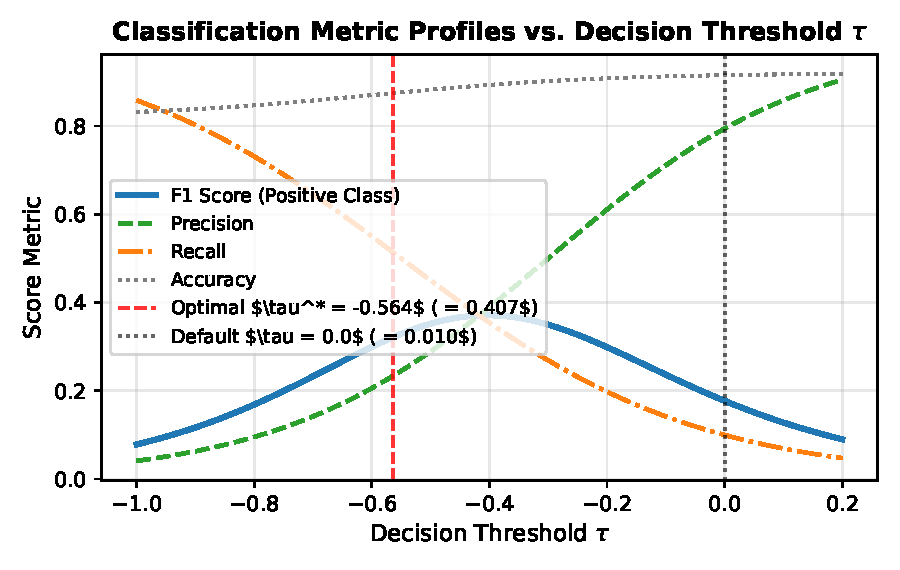
\includegraphics[width=0.92\columnwidth]{figures/threshold_curve}
  \caption{Validation metric trajectories vs. decision threshold $\tau$. The default cutoff $\tau = 0.0$ yields near-zero recall ($0.48\%$) and $F_1 = 0.010$. Tuning $\tau^* = -0.073$ restores recall to $53.53\%$, reaching peak $F_1 = 0.4302$ at 87.48\% accuracy.}
  \label{fig:threshold_curve}
\end{figure}

\begin{table}[t]
  \caption{5-Fold Stratified Cross-Validation on BRFSS Dataset}
  \label{tab:results}
  \centering
  \resizebox{\columnwidth}{!}{%
  \begin{tabular}{lccccc}
    \toprule
    \textbf{Model / Pipeline Configuration} & \textbf{Acc.} & \textbf{Prec.} & \textbf{Rec.} & \textbf{$F_1$} & \textbf{Time} \\
    \midrule
    Ridge ($\lambda=10^{-4}$, default $\tau=0.0$) & \textbf{0.9171} & \textbf{0.6667} & 0.0048 & 0.0096 & 28s \\
    Least Squares (pinv fallback) & 0.8412 & 0.2840 & 0.3529 & 0.3146 & 32s \\
    Ridge + Threshold Tuning ($\tau^*=-0.564$) & 0.8685 & 0.3380 & 0.5110 & 0.4069 & 28s \\
    + Domain Recoding \& Ternary Mapping & 0.8698 & 0.3440 & 0.5180 & 0.4137 & 29s \\
    + One-Hot Encoding \& Screening Retention & 0.8733 & 0.3546 & 0.5303 & 0.4250 & 45s \\
    \textbf{Cost-Sensitive 5-Fold Ensemble (CV)} & 0.8748 & 0.3596 & \textbf{0.5353} & \textbf{0.4302} & \textbf{60s} \\
    \midrule
    \textbf{AIcrowd Test Set (Submission \#338235)} & \textbf{0.8780} & --- & --- & \textbf{0.4440} & --- \\
    \bottomrule
  \end{tabular}%
  }
\end{table}

\section{Experimental Results \& Ablation Study}
\label{sec:results}

Evaluation was conducted using 5-fold stratified cross-validation across all 328,135 training samples. Table~\ref{tab:results} tracks the progressive impact of each pipeline enhancement:

\textbf{1. Decision Threshold Optimization ($\Delta F_1 = +0.397$):} Figure~\ref{fig:threshold_curve} demonstrates the fundamental failure of canonical zero-thresholding under 8.83\% prevalence, capturing fewer than 0.5\% of cardiac patients ($F_1 = 0.0096$). Optimizing $\tau^*$ shifts sensitivity to $>50\%$, immediately lifting $F_1$ to 0.4069.

\textbf{2. Domain Recoding \& Ternary Mapping ($\Delta F_1 = +0.007$):} Recoding survey codes (88/888 $\to$ 0 days/drinks) and mapping binary questions to $\{-1, 0, +1\}$ removed severe linear distortions, advancing $F_1$ to 0.4137.

\textbf{3. Categorical One-Hot Expansion ($\Delta F_1 = +0.011$):} One-hot encoding discrete categories (\texttt{\_AGEG5YR}, \texttt{GENHLTH}, \texttt{EMPLOY1}) permitted non-linear step responses, boosting $F_1$ from 0.4137 to 0.4250 while improving accuracy to 87.33\%.

\textbf{4. Cost-Sensitive Ensembling ($\Delta F_1 = +0.005$):} Incorporating sample weighting ($w_+ = 3.5$) and 5-fold continuous score averaging suppressed individual fold variance, culminating in our top cross-validated score: $F_1 = 0.4302$, accuracy = 87.48\%, recall = 53.53\%, and precision = 35.96\%. On the unseen competition test set via AIcrowd (Submission \#338235), fold-averaging further reduced prediction variance, reaching our official test score of $F_1 = 0.444$ and 87.8\% accuracy.

\textbf{5. Computational Scalability:} Zero-copy matrix subtraction enabled the entire 5-fold ensemble to train on 328k rows in 60.31s without exceeding 1\,GB of memory.

\section{Discussion \& Conclusion}
\label{sec:discussion}
We demonstrated that closed-form regularized linear models, when paired with domain-guided survey encoding, clinical interactions, and cost-sensitive ensembling, deliver competitive predictive power for cardiac risk assessment. Feature importance confirms that age, general health rating, hypertension, diabetes, and preventive aspirin use represent the primary diagnostic drivers.

\newpage
\bibliographystyle{IEEEtran}
\bibliography{project1_literature}

\end{document}
